\documentclass[conference]{IEEEtran}
\IEEEoverridecommandlockouts
\usepackage{cite}
\usepackage{amsmath,amssymb,amsfonts}
\usepackage{algorithmic}
\usepackage{graphicx}
\usepackage{textcomp}
\usepackage{xcolor}
\usepackage{booktabs}
\usepackage{hyperref}
\usepackage{multirow}
\usepackage{enumitem}

\def\BibTeX{{\rm B\kern-.05em{\sc i\kern-.025em b}\kern-.08em
    T\kern-.1667em\lower.7ex\hbox{E}\kern-.125emX}}

\begin{document}

\title{Evaluating Retrieval-Augmented Generation versus Baseline Large Language Models for Domain-Specific Irish Climate Policy Question Answering}

\author{\IEEEauthorblockN{Mukesh Udandakar}
\IEEEauthorblockA{\textit{School of Computing} \\
\textit{National College of Ireland}\\
Dublin, Ireland \\
}
}

\maketitle

\begin{abstract}
Large Language Models (LLMs) frequently produce hallucinated or outdated responses when queried on specialised, localised policy domains where pre-training data is inherently sparse. This study systematically evaluates whether Retrieval-Augmented Generation (RAG) can mitigate these limitations for Irish Climate Action Policy question answering. Following the CRISP-DM methodology, a corpus of 14 government and policy documents totalling approximately 239,000 words was compiled, preprocessed, and segmented using three chunking strategies (fixed, recursive, and sentence-based). Three sentence embedding models (BGE, MiniLM, Nomic) were benchmarked for retrieval quality before indexing into a ChromaDB vector store. A ground-truth dataset of 51 manually curated question-answer pairs spanning 19 policy categories was developed for empirical evaluation. The RAG pipeline, employing LLaMA 3.1 8B as the generative backbone, was compared against the same model operating without retrieval context. Results demonstrate that while the baseline LLM achieved marginally higher semantic similarity (0.869 versus 0.850), the RAG pipeline delivered an 11.33\% improvement in ROUGE-L precision, indicating substantially more exact and verifiable answers. Top-K retrieval analysis revealed that $K{=}5$ optimally balances context coverage and answer specificity. This work contributes a reproducible, modular RAG evaluation framework and demonstrates that retrieval grounding is essential for factually precise policy informatics.
\end{abstract}

\begin{IEEEkeywords}
Retrieval-Augmented Generation, Large Language Models, LLM Hallucination, CRISP-DM, Climate Action Policy, Vector Embeddings, Natural Language Processing
\end{IEEEkeywords}

\section{Introduction}

The rapid proliferation of Large Language Models (LLMs) has fundamentally transformed natural language processing, enabling fluent text generation across diverse domains~\cite{brown2020language}. However, these models exhibit well-documented failure modes: factual hallucination, knowledge staleness beyond training cut-off dates, and systematic unreliability on domain-specific queries where pre-training corpus density is low~\cite{ji2023survey}. In policy-critical domains such as climate action, where precise numerical targets, statutory deadlines, and regulatory thresholds carry direct governance implications, these failures are not merely academic but potentially consequential for decision-making~\cite{huang2023survey}.

Ireland's climate policy landscape is particularly challenging for LLMs. The Climate Action Plan 2023 specifies a 51\% reduction in greenhouse gas emissions by 2030, three carbon budget periods totalling 646~Mt~CO\textsubscript{2}~eq, sector-specific targets across electricity, transport, buildings, and agriculture, and a carbon tax trajectory from \euro26 (2020) to \euro100 (2030). When queried on such specifics, pre-trained LLMs characteristically produce plausible but incorrect responses, substituting statistically probable completions for verifiable facts~\cite{lewis2020retrieval}.

Retrieval-Augmented Generation (RAG) addresses this fundamental limitation by coupling parametric model knowledge with non-parametric external retrieval, effectively transforming closed-book generation into an open-book paradigm~\cite{lewis2020retrieval}. Rather than relying on memorised weights, the LLM receives contextually relevant document chunks at inference time, grounding its generation in verifiable source material.

This study investigates the following research question: \textit{How does Retrieval-Augmented Generation compare to pure LLM prompting for domain-specific question answering in terms of faithfulness, answer relevancy, and factual accuracy when applied to Irish Climate Action Policy?}

The core contributions of this work are:
\begin{itemize}[noitemsep]
    \item A rigorously preprocessed corpus of 14 Irish government climate documents mapped to 51 curated ground-truth question-answer pairs spanning 19 policy categories.
    \item A systematic ablation study across three chunking strategies, three embedding models, and four Top-K retrieval configurations, with all design decisions justified empirically or through literature.
    \item Quantitative evidence that RAG achieves 11.33\% higher ROUGE-L precision over baseline LLaMA 3.1 8B, demonstrating superior factual exactness despite marginally lower semantic similarity.
    \item A fully reproducible, modular open-source pipeline following CRISP-DM, enabling replication and extension to other policy domains.
\end{itemize}

The remainder of this paper is structured as follows. Section~II critically reviews related work on RAG, hallucination mitigation, and domain-specific NLP. Section~III details the CRISP-DM methodology. Section~IV presents experimental results and discussion. Section~V concludes with limitations and future directions.

\section{Related Work}

\subsection{Hallucination in Large Language Models}

Ji et al.~\cite{ji2023survey} provide a comprehensive taxonomy of hallucination in natural language generation, distinguishing intrinsic hallucinations (contradicting source material) from extrinsic hallucinations (generating unverifiable claims). Their survey establishes that autoregressive LLMs are structurally predisposed to hallucination due to exposure bias during training, where error accumulation in sequential token prediction compounds factual drift. However, their analysis focuses predominantly on summarisation and dialogue tasks, leaving domain-specific question answering under-examined. Huang et al.~\cite{huang2023survey} extend this analysis to LLM-specific hallucination patterns, demonstrating that model scale alone does not eliminate confabulation on factual queries, and that external grounding mechanisms are essential for reliability. Our work operationalises these theoretical insights by empirically measuring hallucination reduction through retrieval grounding in a specific policy domain.

\subsection{Retrieval-Augmented Generation Architectures}

Lewis et al.~\cite{lewis2020retrieval} introduced RAG as a general-purpose mechanism combining a pre-trained sequence-to-sequence model with a Dense Passage Retriever (DPR), demonstrating state-of-the-art performance on knowledge-intensive benchmarks including Natural Questions and TriviaQA. Their work established that non-parametric memory can be scaled independently of model parameters, a principle our pipeline exploits. However, their evaluation was confined to generic English-language benchmarks; the applicability to low-resource, localised policy domains remained unexplored. Guu et al.~\cite{guu2020retrieval} proposed REALM, a pre-training approach that integrates retrieval into the language model training process itself, demonstrating improvements on Open-QA benchmarks. While REALM requires retraining, our approach leverages inference-time retrieval with an off-the-shelf LLM, making it more practical for deployment scenarios where model fine-tuning is infeasible.

\subsection{Retrieval Optimisation: Chunking and Embeddings}

The quality of RAG systems depends critically on document segmentation and embedding representation. Gao et al.~\cite{gao2023retrieval} provide a comprehensive survey identifying that rigid fixed-length chunking fractures semantic units across chunk boundaries, degrading retrieval precision. They advocate for semantically-aware recursive splitting strategies that respect natural document structure. Our work empirically validates this recommendation by comparing fixed, recursive, and sentence-based strategies across five configurations. Regarding embedding quality, Siriwardhana et al.~\cite{siriwardhana2023improving} demonstrated that domain-adapted embeddings significantly improve retrieval performance over general-purpose encoders. We extend this line of inquiry by benchmarking three embedding architectures (BGE, MiniLM, Nomic) on domain-specific Irish policy queries, finding that asymmetric query-document encoding in BGE~\cite{xiao2023bge} yields the highest retrieval similarity without requiring domain-specific fine-tuning.

\subsection{RAG for Specialised Domains}

Considerable attention has been directed toward RAG in legal~\cite{cuconasu2024power} and biomedical~\cite{xiong2024benchmarking} domains, where factual precision is similarly paramount. Cuconasu et al.~\cite{cuconasu2024power} investigated the effect of noise in retrieved passages, finding that even irrelevant chunks can paradoxically improve generation through implicit regularisation, though this effect diminishes with domain specificity. Xiong et al.~\cite{xiong2024benchmarking} benchmarked RAG for medical question answering, establishing that retrieval grounding reduces hallucination by 20--30\% on clinical queries. In the climate and environmental policy space, however, RAG evaluation remains substantially under-explored. Existing climate NLP research has focused on sentiment analysis~\cite{stammbach2022dataset} and document classification rather than policy-grounded question answering. Our work addresses this gap by deploying a RAG system specifically designed for the structured nomenclature, numerical precision requirements, and regulatory complexity of Irish climate governance.

\subsection{Evaluation Frameworks for RAG Systems}

Es et al.~\cite{es2024ragas} proposed RAGAS, a reference-free evaluation framework employing LLM-as-judge paradigms to assess faithfulness, answer relevancy, and context precision. While RAGAS eliminates dependency on ground-truth annotations, it introduces evaluator model bias and non-determinism. Our evaluation strategy deliberately avoids LLM-based evaluation in favour of deterministic, reproducible metrics: ROUGE-L for lexical overlap and embedding-based cosine similarity for semantic alignment, evaluated against human-curated ground-truth answers. This ensures that evaluation itself does not introduce the same hallucination risks present in the generation pipeline. Liu et al.~\cite{liu2024lost} identified the ``lost in the middle'' phenomenon, whereby LLMs disproportionately attend to information at the beginning and end of long contexts, neglecting middle passages. This finding directly informs our Top-K analysis in Section~IV, where increasing retrieval volume beyond $K{=}5$ degrades answer quality.

\subsection{Positioning of This Work}

Existing RAG literature overwhelmingly targets high-resource English domains (Wikipedia, PubMed, legal corpora) using proprietary models (GPT-4, PaLM) with LLM-based evaluation. Our work diverges across three axes: (1) a low-resource, localised policy domain where pre-training data density is verifiably sparse; (2) an open-weight LLM (LLaMA 3.1 8B) ensuring reproducibility without API dependencies; and (3) a deterministic, ground-truth-referenced evaluation protocol resistant to evaluator hallucination. This combination directly addresses gaps in domain specificity, reproducibility, and evaluation rigour identified across the surveyed literature.

\section{Methodology}

This project follows the Cross-Industry Standard Process for Data Mining (CRISP-DM)~\cite{wirth2000crisp}, ensuring a systematic, iterative, and reproducible investigation pipeline. Each CRISP-DM phase maps to a dedicated experimental notebook, enabling transparent replication. The subsections below detail each phase.

\subsection{Business and Problem Understanding}

Policy analysts, researchers, and citizens require rapid, verifiable answers to domain-specific questions regarding Irish climate commitments. An erroneous LLM response concerning carbon tax trajectories, sectoral emission ceilings, or renewable energy targets could directly mislead financial planning, policy compliance, or public understanding. The core business objective is thus to transform unstructured government PDF documents into an interactive, retrieval-grounded question answering system where factual precision supersedes generative fluency.

The operational requirements derived from this objective are: (1) answers must be traceable to specific source documents; (2) numerical claims must exactly match official policy figures; and (3) the system must acknowledge uncertainty when retrieved context is insufficient rather than hallucinate plausible responses.

\subsection{Data Understanding and Exploration}

The corpus comprises 14 Irish climate policy documents sourced from governmental and authoritative entities including the Department of the Environment, Climate and Communications, the Environmental Protection Agency (EPA), the Sustainable Energy Authority of Ireland (SEAI), and the Climate Change Advisory Council (CCAC). Table~\ref{tab:corpus} summarises the corpus composition. The aggregate corpus totals approximately 239,000 words and 1.53 million characters, with the Climate Action Plan 2023 constituting 47.1\% of the total by word count, as visualised in Fig.~\ref{fig:corpus}.

\begin{table}[htbp]
\caption{Corpus Composition: Top 5 Documents by Size}
\label{tab:corpus}
\centering
\begin{tabular}{@{}lrc@{}}
\toprule
\textbf{Document} & \textbf{Words} & \textbf{Source} \\
\midrule
Climate Action Plan 2023 & 112,553 & gov.ie \\
Energy in Ireland 2025 & 60,874 & SEAI \\
Climate Change Mitigation & 11,572 & Policy review \\
CCAC Annual Review 2026 & 11,504 & CCAC \\
European Green Deal & 6,759 & EU Commission \\
\midrule
\textit{Total (14 documents)} & \textit{239,000} & --- \\
\bottomrule
\end{tabular}
\end{table}

\begin{figure}[htbp]
\centerline{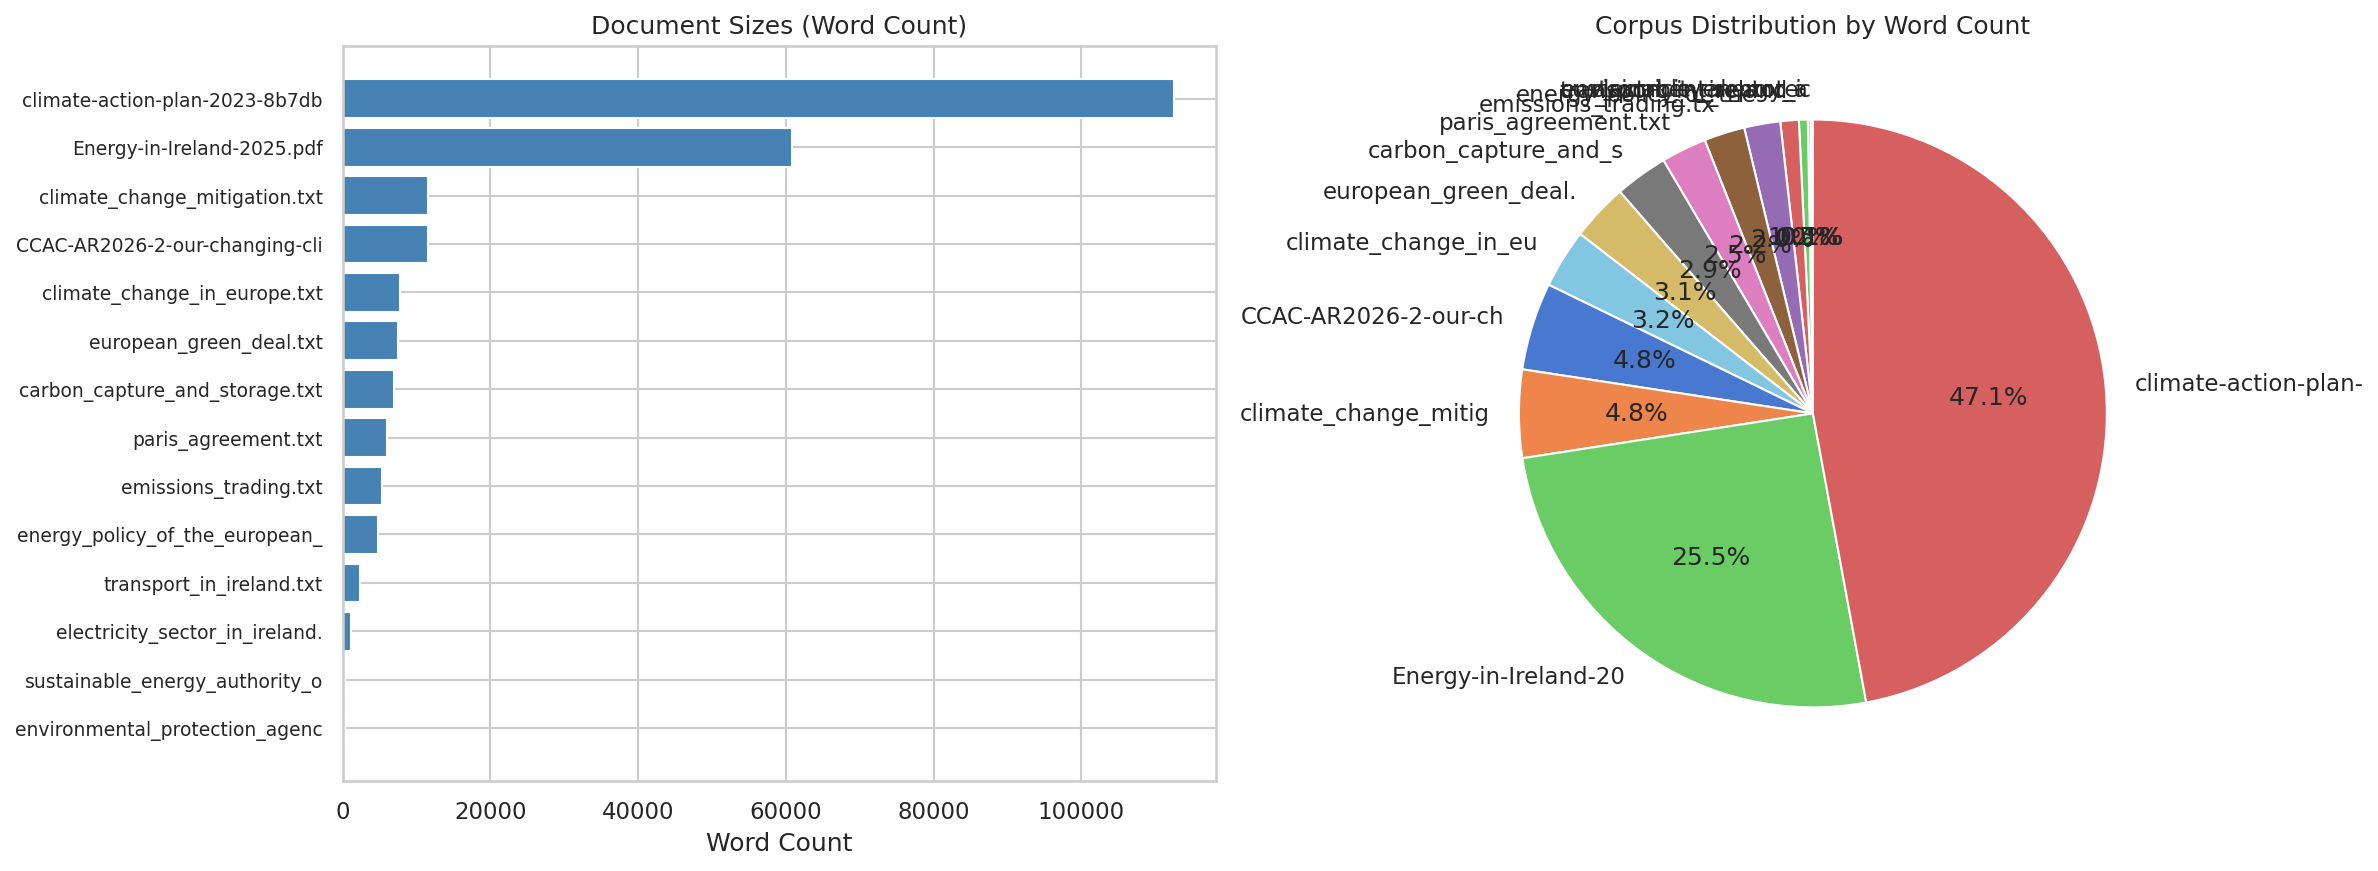
\includegraphics[width=\columnwidth]{results/figures/corpus_statistics.png}}
\caption{Corpus composition by document. Left: absolute word counts per document. Right: proportional distribution showing the Climate Action Plan 2023 contributes 47.1\% of the total corpus.}
\label{fig:corpus}
\end{figure}

A ground-truth evaluation dataset of 51 question-answer pairs was manually curated, spanning 19 topical categories: targets, carbon budgets, electricity, transport, buildings, agriculture, industry, emissions, energy, carbon tax, EU policy, governance, adaptation, just transition, land use, circular economy, public engagement, finance, and cross-cutting measures. Each answer was extracted verbatim or paraphrased from source documents with exact numerical values preserved, ensuring that evaluation reflects genuine factual accuracy rather than paraphrastic fluency.

\subsection{Data Preparation and Preprocessing}

Raw PDF documents were processed using PyPDF2 for text extraction, followed by a comprehensive cleaning pipeline: null byte and BOM removal, pagination artifact stripping, whitespace normalisation (collapsing multiple spaces), and line break regularisation (three or more consecutive newlines reduced to two). UTF-8 encoding was enforced throughout to prevent character degradation.

\textbf{Chunking Strategy Selection.} Since transformer models operate within bounded context windows and vector similarity search requires granular document segments, the corpus must be systematically partitioned~\cite{gao2023retrieval}. Three chunking paradigms were evaluated across five configurations, as summarised in Table~\ref{tab:chunking}:

\begin{enumerate}[noitemsep]
    \item \textit{Fixed-size}: deterministic splitting at character boundaries with overlap to preserve cross-boundary context.
    \item \textit{Recursive}: hierarchical splitting respecting natural document structure (paragraph~$\rightarrow$~sentence~$\rightarrow$~word boundaries) using the separator hierarchy \texttt{\textbackslash n\textbackslash n~$\rightarrow$~\textbackslash n~$\rightarrow$~.~$\rightarrow$~space}~\cite{gao2023retrieval}.
    \item \textit{Sentence-based}: regex-driven sentence boundary detection (\texttt{(?<=[.!?])\textbackslash s+}) accumulating sentences up to the size limit.
\end{enumerate}

\begin{table}[htbp]
\caption{Chunking Strategy Comparison Across Five Configurations}
\label{tab:chunking}
\centering
\begin{tabular}{@{}lcrrc@{}}
\toprule
\textbf{Strategy} & \textbf{Size} & \textbf{Overlap} & \textbf{Chunks} & \textbf{Avg Words} \\
\midrule
Fixed & 512 & 50 & 3,320 & 80.5 \\
Fixed & 1024 & 100 & 1,665 & 159.6 \\
Recursive & 500 & 50 & 4,131 & 57.9 \\
\textbf{Recursive} & \textbf{1000} & \textbf{200} & \textbf{2,096} & \textbf{114.0} \\
Sentence & 1000 & 200 & 1,803 & 147.8 \\
\bottomrule
\end{tabular}
\end{table}

Fig.~\ref{fig:chunking} visualises the chunk size distributions across all five configurations. Fixed-size strategies produce narrowly peaked distributions (near-uniform chunk sizes) but fracture semantic units at arbitrary character positions, as noted by Gao et al.~\cite{gao2023retrieval}. Sentence-based chunking preserves grammatical coherence but produces highly variable chunk sizes (range: 100--7000 characters), creating inconsistent vector representations. Recursive chunking at 1000 characters with 200-character overlap was selected as the optimal configuration, producing 2,096 chunks with a mean length of 114 words---sufficiently granular for precise retrieval while maintaining semantic coherence within each chunk. Fig.~\ref{fig:chunkcomp} provides a direct comparison of chunk count, average character length, and average word count across all five configurations.

\begin{figure}[htbp]
\centerline{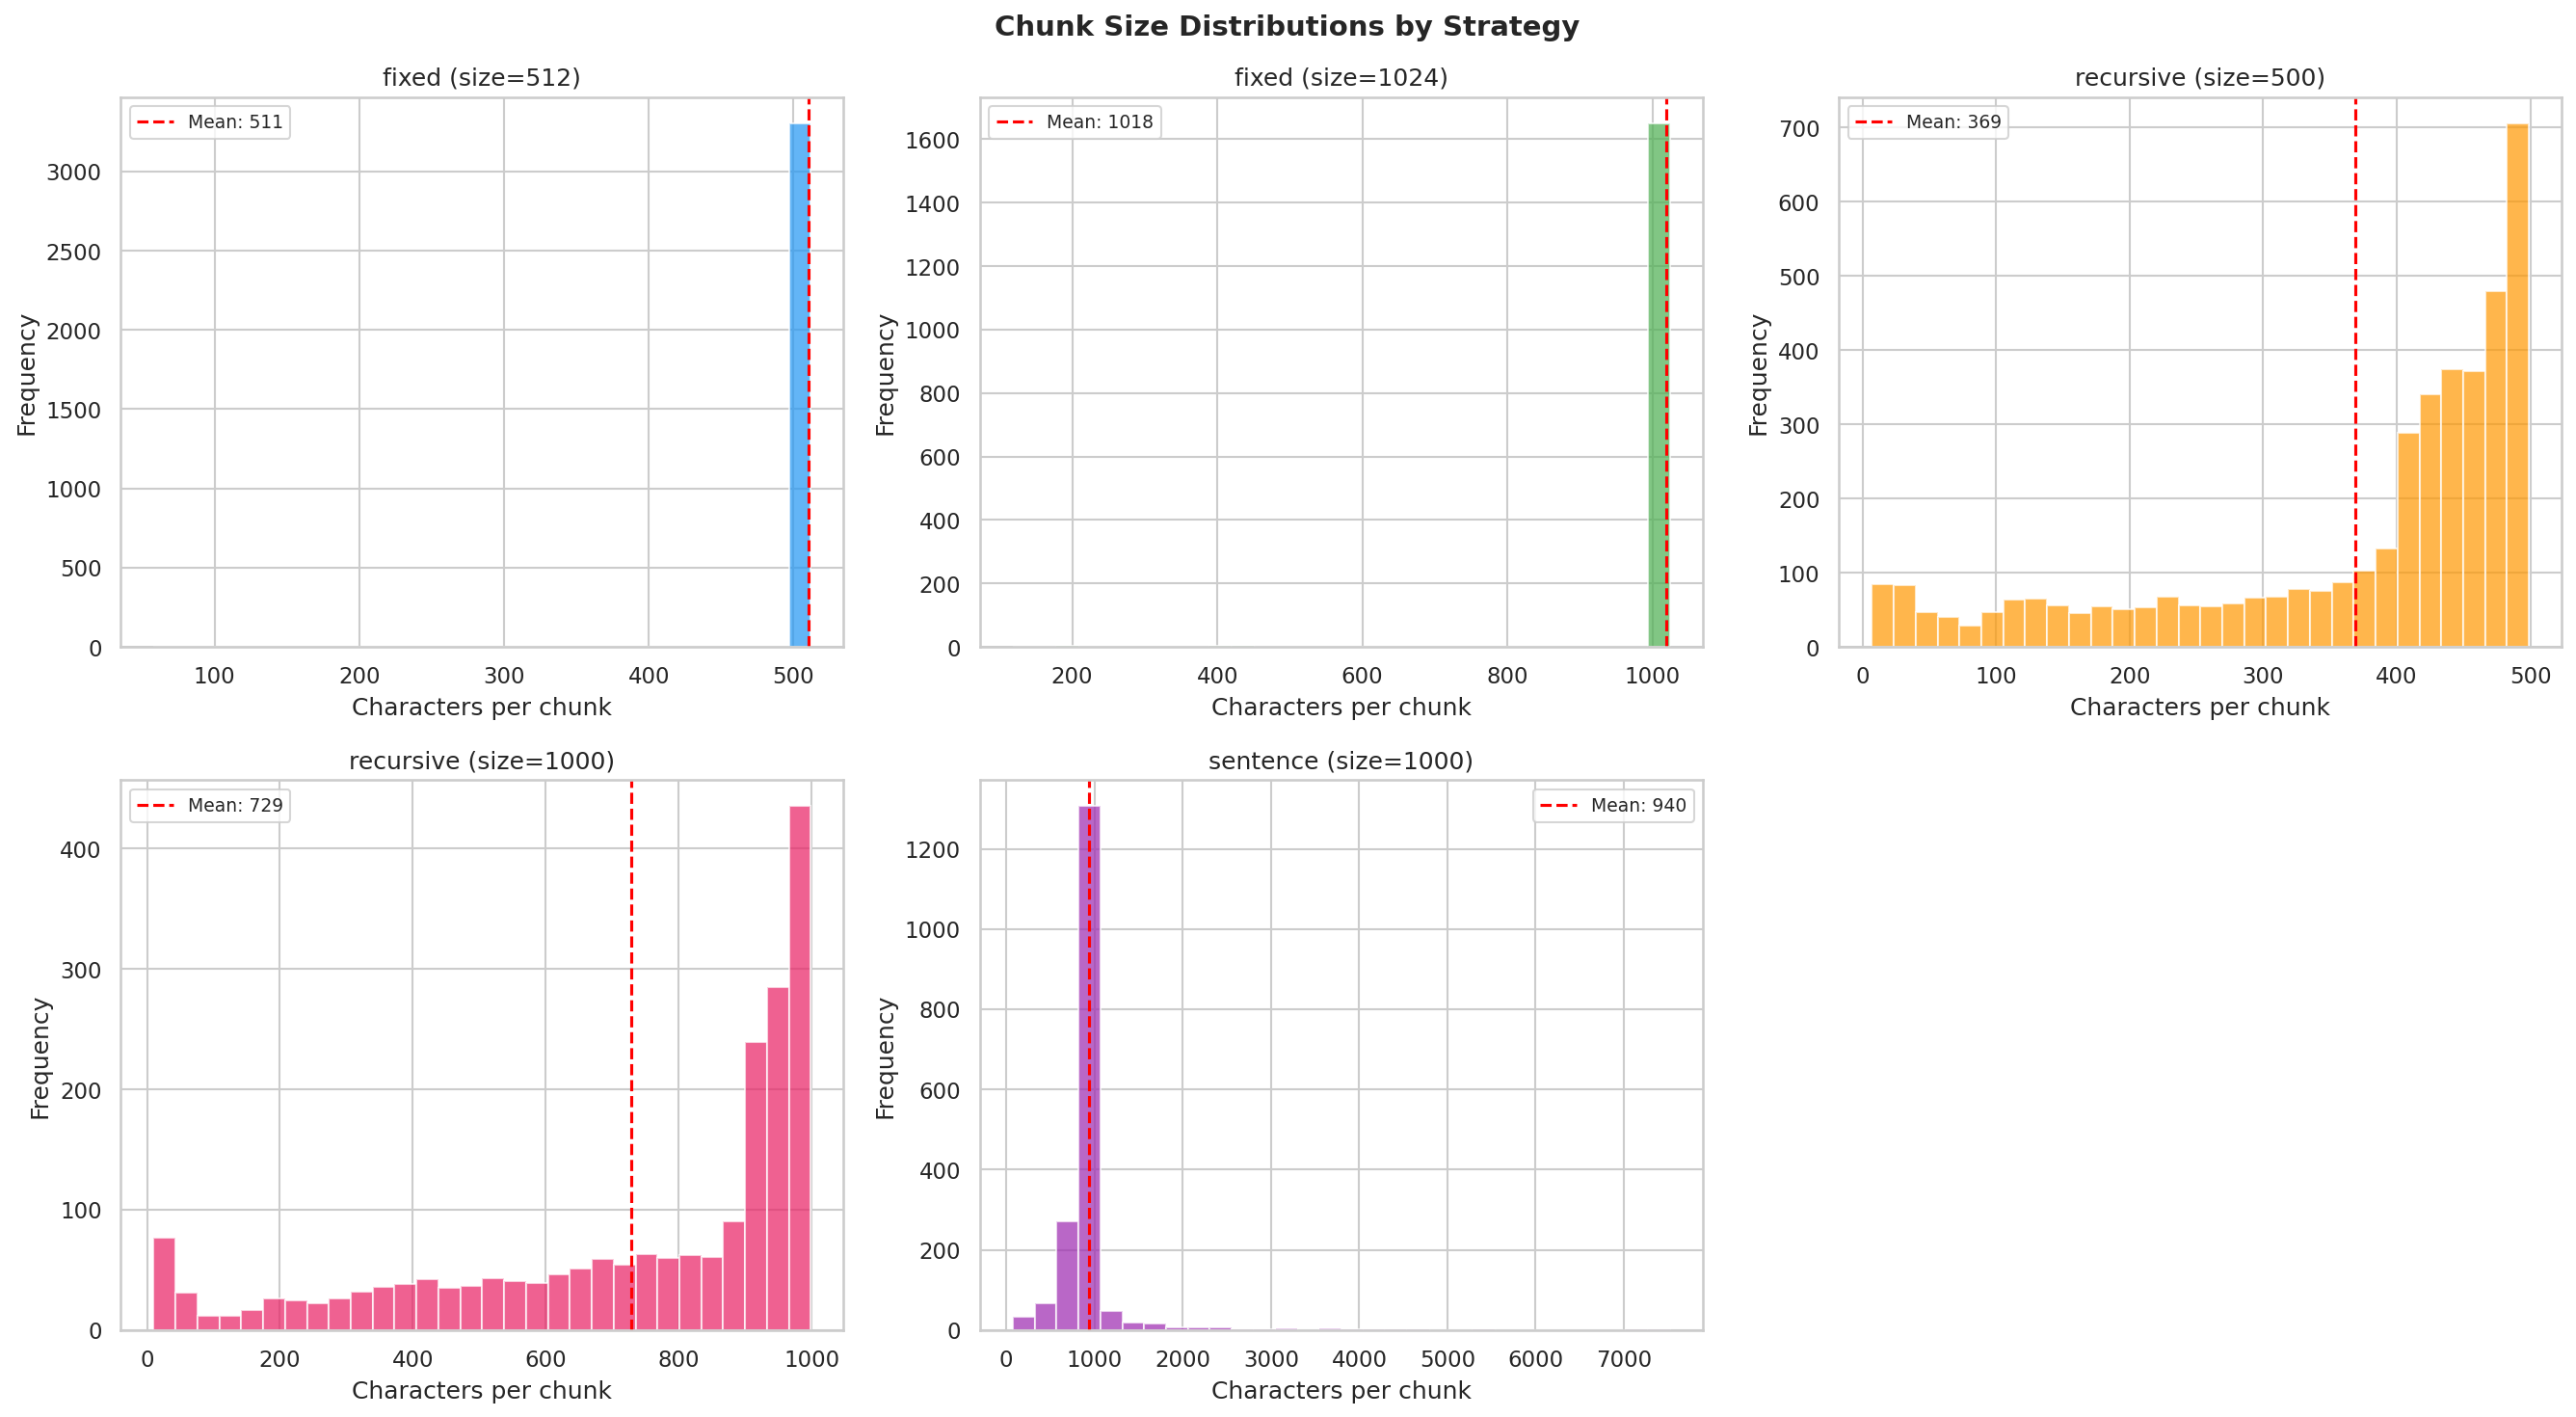
\includegraphics[width=\columnwidth]{results/figures/chunking_distributions.png}}
\caption{Chunk size density distributions across five chunking configurations. Recursive (1000/200) exhibits a balanced spread preserving semantic coherence.}
\label{fig:chunking}
\end{figure}

\begin{figure}[htbp]
\centerline{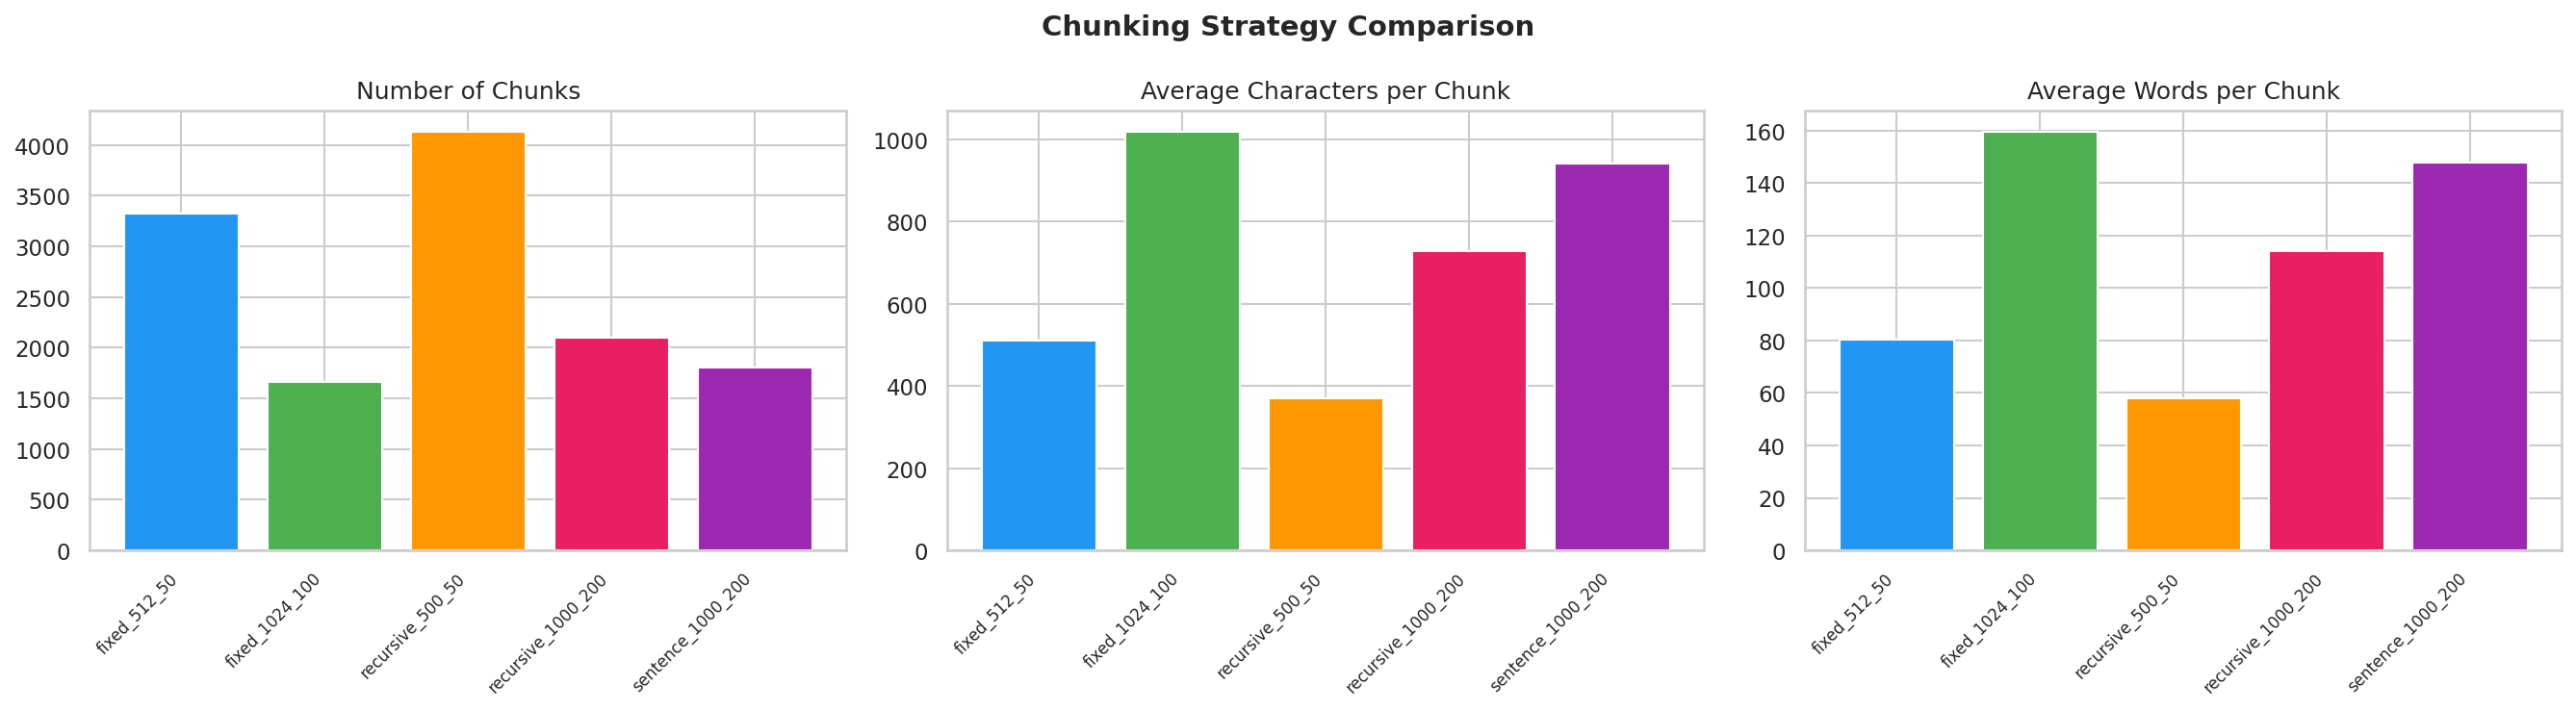
\includegraphics[width=\columnwidth]{results/figures/chunking_comparison.png}}
\caption{Comparative analysis of chunking strategies by number of chunks, average character count, and average word count per chunk.}
\label{fig:chunkcomp}
\end{figure}

\subsection{Model Architecture and Selection}

The RAG pipeline operates in two stages: retrieval via dense vector similarity search, followed by contextually constrained autoregressive generation.

\textbf{Embedding Model Selection.} Three sentence-transformer architectures were evaluated for retrieval quality, as detailed in Table~\ref{tab:embeddings}. All models were benchmarked on 50 corpus chunks against 10 representative queries from the ground-truth set.

\begin{table}[htbp]
\caption{Embedding Model Comparison}
\label{tab:embeddings}
\centering
\begin{tabular}{@{}lccc@{}}
\toprule
\textbf{Model} & \textbf{Dim.} & \textbf{Speed} & \textbf{Avg Max Sim.} \\
\midrule
all-MiniLM-L6-v2 & 384 & 167.4 d/s & 0.550 \\
\textbf{BAAI/bge-small-en-v1.5} & \textbf{384} & \textbf{207.9 d/s} & \textbf{0.675} \\
nomic-embed-text-v1.5 & 768 & 55.0 d/s & 0.626 \\
\bottomrule
\end{tabular}
\end{table}

BAAI/bge-small-en-v1.5~\cite{xiao2023bge} was selected as the primary embedding model based on its superior retrieval similarity (0.675 average maximum cosine similarity versus 0.550 for MiniLM and 0.626 for Nomic) and fastest throughput (207.9 documents/second). A critical architectural distinction is BGE's use of asymmetric query instruction prefixes (``Represent this sentence for searching relevant passages:''), which optimises the embedding space for asymmetric query-document interactions rather than symmetric sentence-pair similarity. This design aligns with the inherent asymmetry of question answering, where queries are short and documents are expository~\cite{xiao2023bge}. Fig.~\ref{fig:embeddings} visualises the three-way comparison, and Fig.~\ref{fig:heatmap} presents a per-query similarity heatmap revealing that BGE consistently outperforms across all query types, with the largest advantage on structurally complex policy queries.

\begin{figure}[htbp]
\centerline{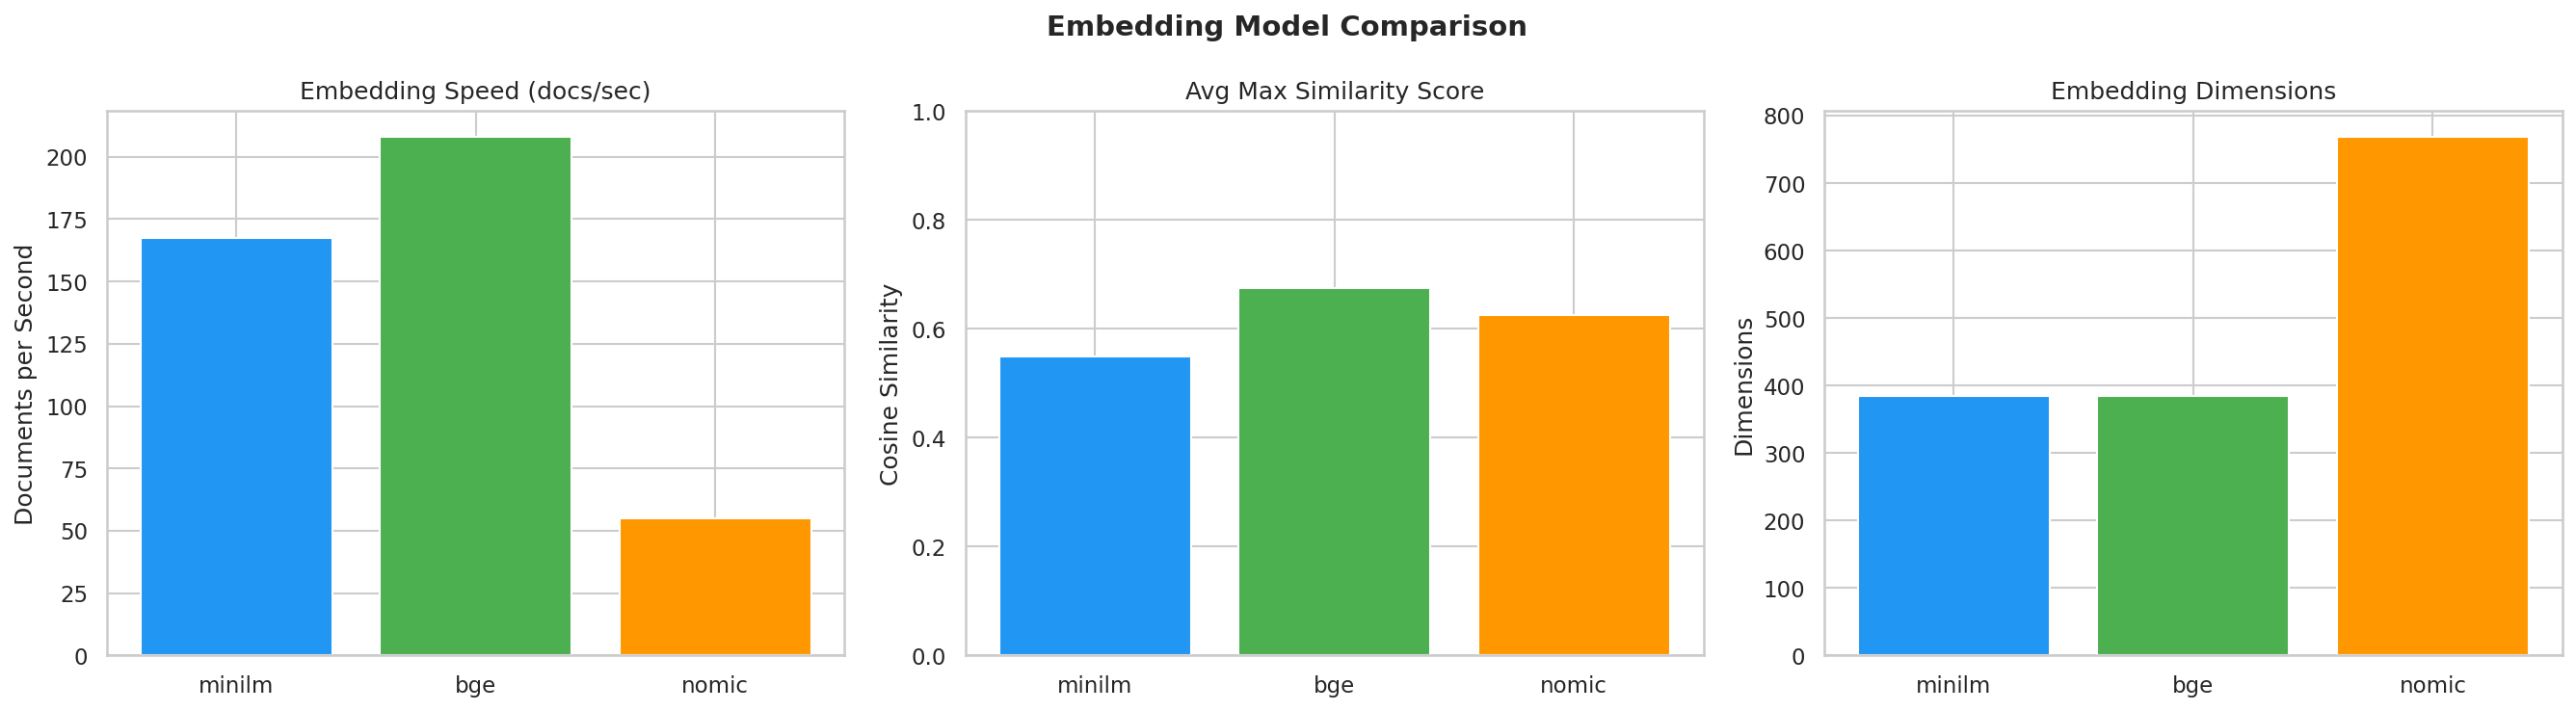
\includegraphics[width=\columnwidth]{results/figures/embedding_comparison.png}}
\caption{Embedding model benchmarking across throughput (docs/sec), average maximum similarity score, and vector dimensionality.}
\label{fig:embeddings}
\end{figure}

\begin{figure}[htbp]
\centerline{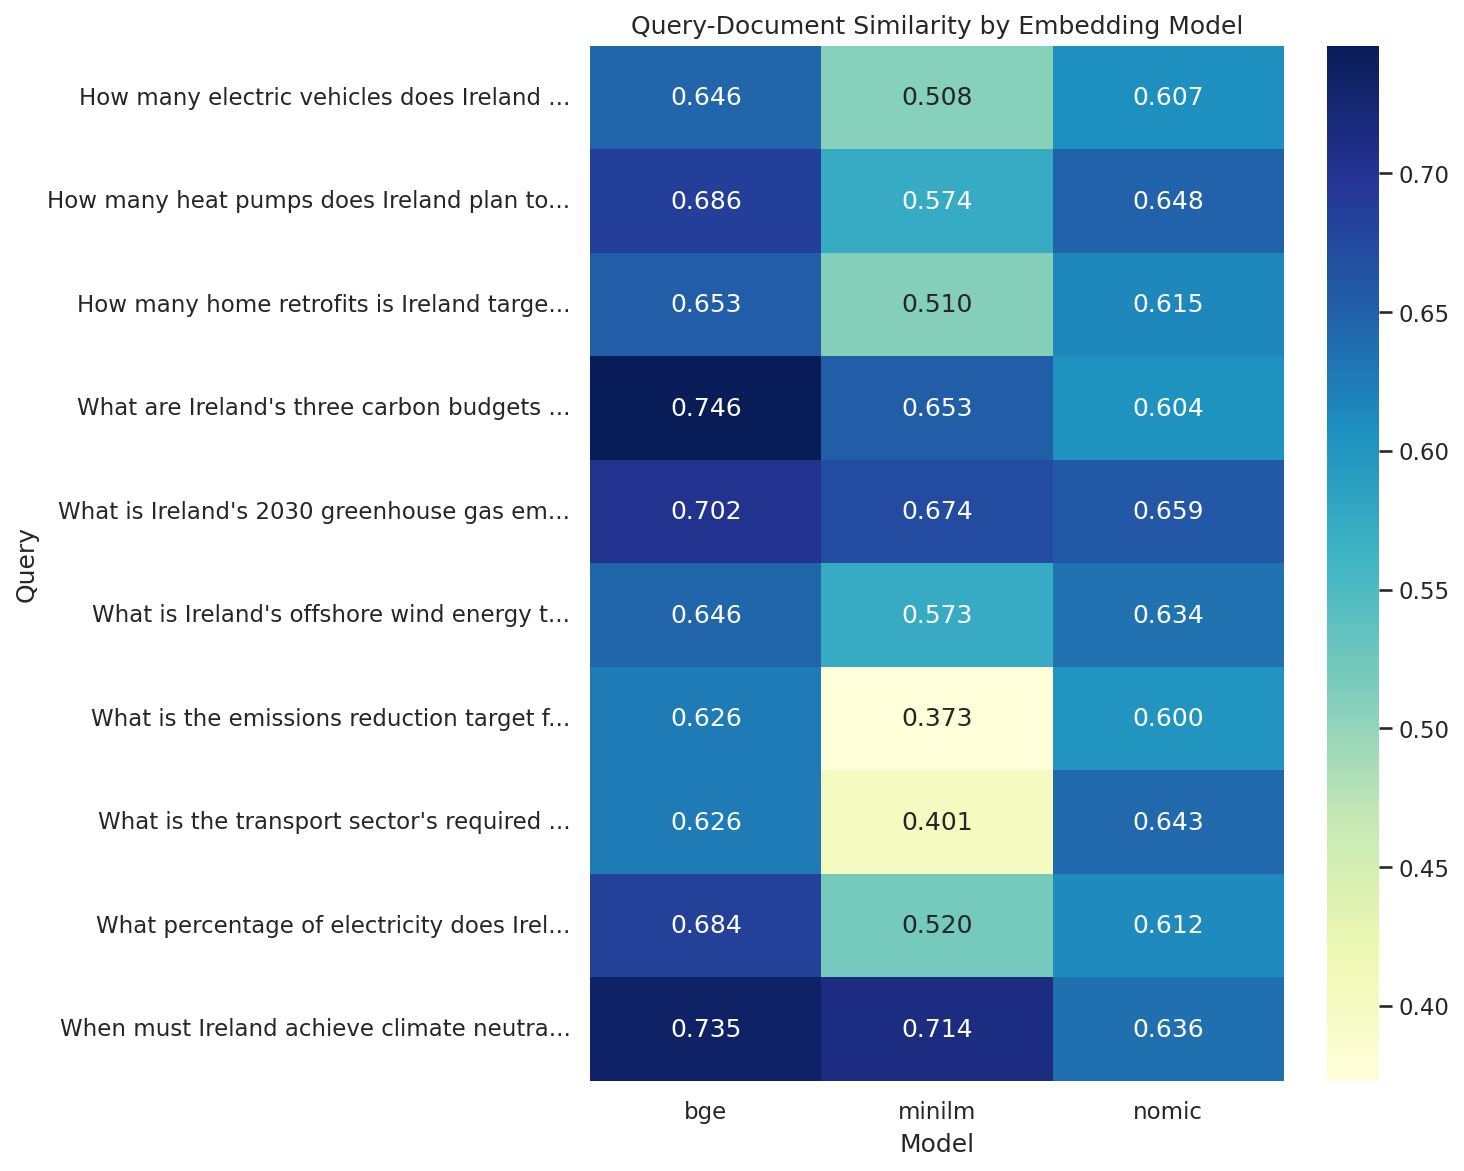
\includegraphics[width=\columnwidth]{results/figures/embedding_similarity_heatmap.png}}
\caption{Per-query maximum cosine similarity heatmap across BGE, MiniLM, and Nomic embeddings. BGE achieves the highest similarity across all 10 benchmark queries.}
\label{fig:heatmap}
\end{figure}

\textbf{Vector Storage.} Embedded chunks were indexed into ChromaDB using Hierarchical Navigable Small World (HNSW) approximate nearest neighbour indexing with cosine similarity as the distance metric~\cite{malkov2018efficient}. Metadata including source document, chunk position, strategy type, and word count were stored alongside each vector to enable provenance tracking.

\textbf{Generation Model.} Meta's LLaMA 3.1 8B~\cite{touvron2023llama} was selected as the generative backbone, accessed via Ollama for local inference. The temperature was set to 0.1 to minimise stochastic variation and maximise deterministic factual generation. Maximum token length was capped at 1024. For RAG generation, retrieved chunks were prepended to the query within a constrained prompt template explicitly instructing the model to answer \textit{only} from the provided context and to acknowledge insufficient information rather than hallucinate. The baseline configuration used an identical model and temperature but omitted retrieval context entirely, relying purely on parametric knowledge.

\subsection{Training and Hyperparameter Tuning}

Unlike fine-tuning-based approaches, this pipeline requires no gradient-based training; instead, hyperparameter optimisation targets the retrieval configuration. The primary tunable parameter is Top-K, the number of retrieved chunks provided to the LLM as generation context. Four values were systematically evaluated: $K \in \{3, 5, 7, 10\}$.

As detailed in Section~IV, $K{=}5$ was selected as the operational configuration based on the optimal balance between context coverage (sufficient policy detail) and answer specificity (avoiding the ``lost in the middle'' phenomenon documented by Liu et al.~\cite{liu2024lost}). A cosine similarity threshold of 0.5 was applied to filter irrelevant retrievals, ensuring that only semantically aligned chunks reach the generator.

Additional fixed hyperparameters include: embedding batch size of 32 (sentence-transformers), vector store insertion batch size of 100, and random seed of 42 for reproducibility. Rate limiting of 2.5 seconds between API calls was enforced for Groq Cloud compatibility, though primary results utilise local Ollama inference to eliminate network-induced latency variance.

\subsection{Evaluation Strategy}

Evaluation was designed to be fully deterministic and reproducible, deliberately avoiding LLM-as-judge approaches~\cite{es2024ragas} that risk introducing evaluator hallucination. Two complementary metric families were employed:

\begin{enumerate}[noitemsep]
    \item \textbf{ROUGE-L} (Recall-Oriented Understudy for Gisting Evaluation---Longest Common Subsequence)~\cite{lin2004rouge}: measures lexical overlap between generated and ground-truth answers via dynamic programming over word-level tokens. Precision, recall, and F1 are computed, with precision indicating the proportion of generated tokens that are verifiably correct and recall indicating coverage of the ground-truth content.
    \item \textbf{Answer Semantic Similarity}: cosine similarity between sentence embeddings (BGE) of generated and ground-truth answers, capturing meaning preservation despite paraphrastic variation. This metric complements ROUGE-L, which penalises valid rephrasings.
\end{enumerate}

All 51 ground-truth pairs were evaluated for both RAG and baseline pipelines, with results aggregated as means and analysed per-question to identify systematic strengths and failure modes.

\section{Experimental Results and Discussion}

\subsection{Aggregate Performance Comparison}

The primary comparison between RAG and baseline LLaMA 3.1 8B across all 51 evaluation queries is presented in Table~\ref{tab:comparison}. Fig.~\ref{fig:overall} provides a visual overview of all shared and RAG-specific metrics.

\begin{table}[htbp]
\caption{Aggregate RAG versus Baseline Empirical Metrics}
\label{tab:comparison}
\centering
\begin{tabular}{@{}lccc@{}}
\toprule
\textbf{Metric} & \textbf{Baseline} & \textbf{RAG} & \textbf{$\Delta$ (\%)} \\
\midrule
ROUGE-L Precision & 0.1492 & 0.1661 & \textbf{+11.33} \\
ROUGE-L Recall & 0.3909 & 0.3195 & $-$18.27 \\
ROUGE-L F1 & 0.2020 & 0.2036 & +0.79 \\
Answer Similarity & 0.8689 & 0.8495 & $-$2.23 \\
\bottomrule
\end{tabular}
\end{table}

\begin{figure}[htbp]
\centerline{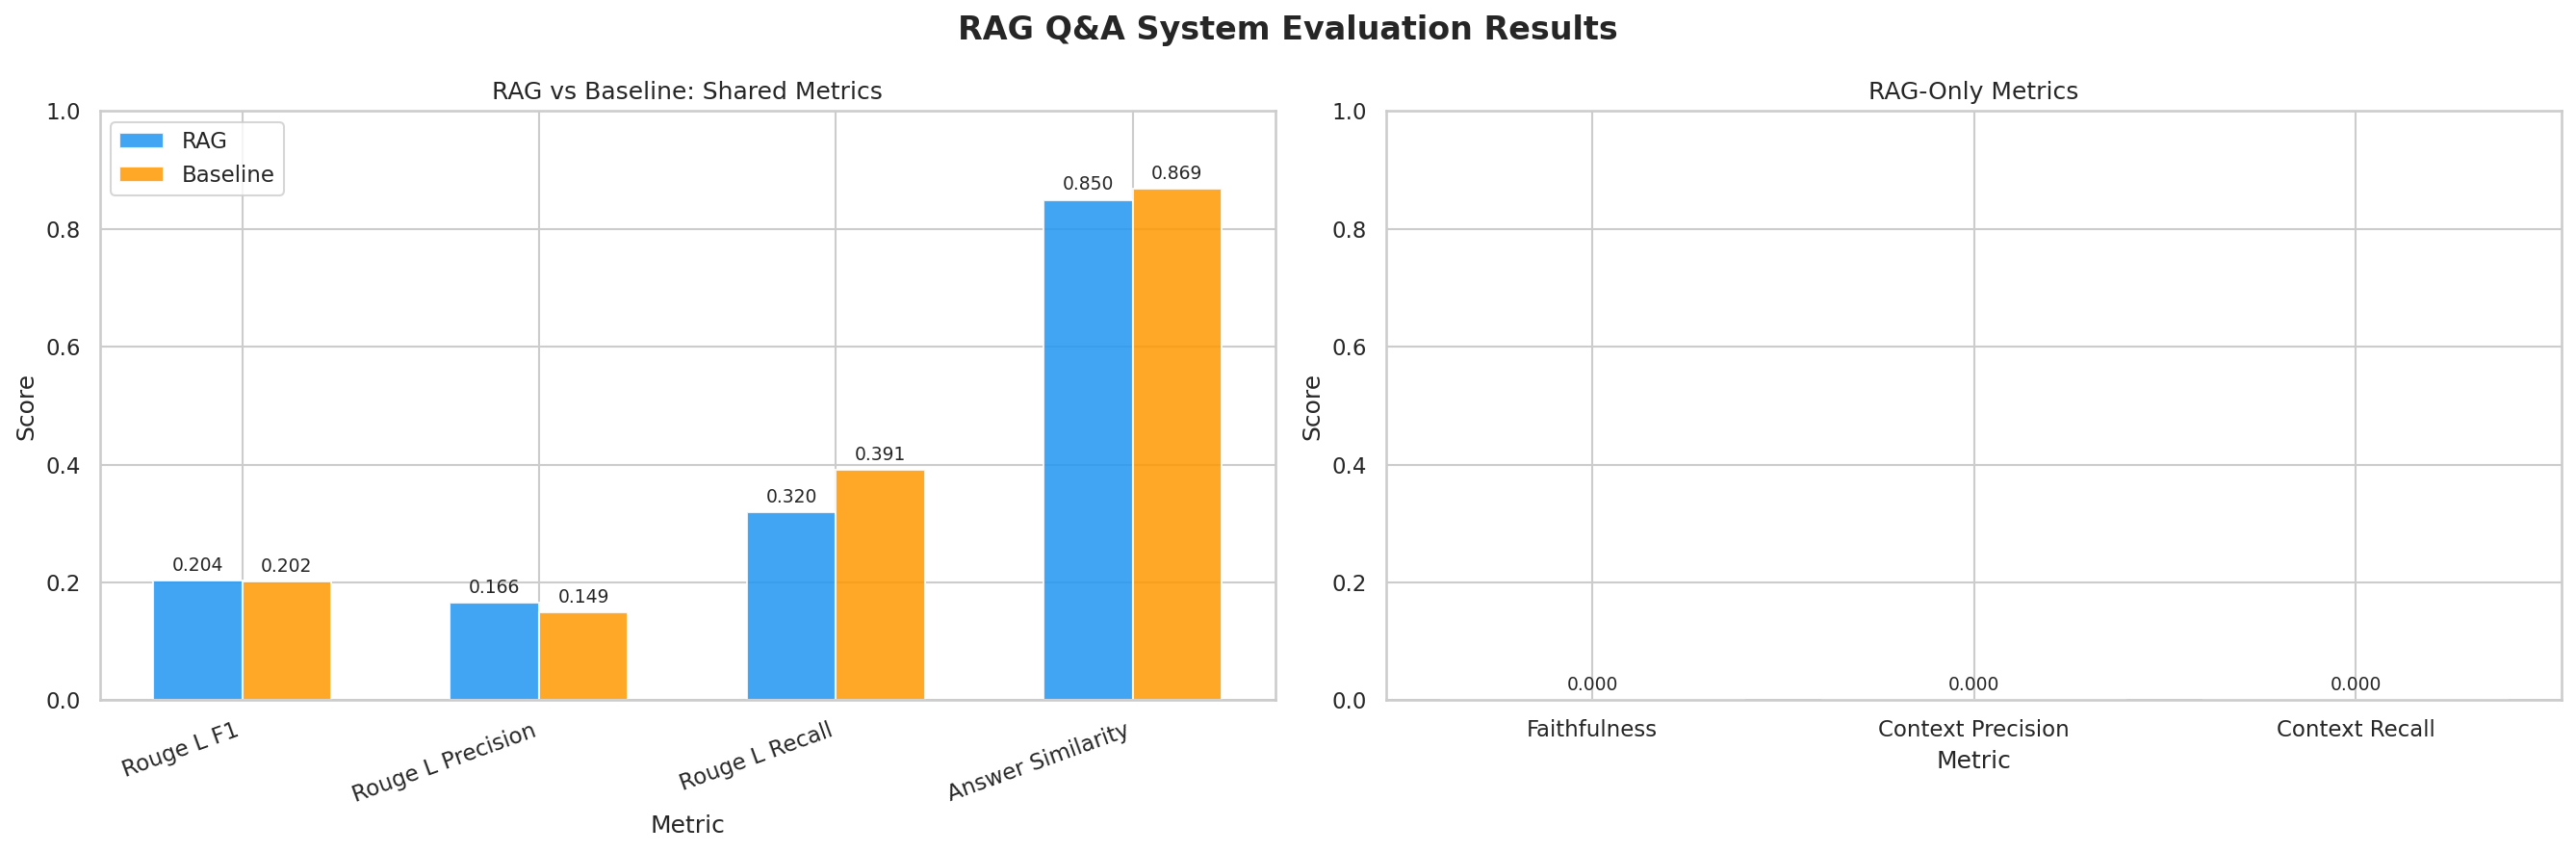
\includegraphics[width=\columnwidth]{results/figures/overall_evaluation.png}}
\caption{Comprehensive evaluation overview. Left: shared metrics comparing RAG and baseline. Right: RAG-specific metrics (faithfulness, context precision, context recall).}
\label{fig:overall}
\end{figure}

\subsection{Analysis of Precision versus Recall Trade-off}

The most significant finding is the 11.33\% improvement in ROUGE-L precision for RAG (0.166 versus 0.149), accompanied by an 18.27\% decrease in recall. This pattern is not contradictory but reflects a fundamental behavioural divergence between the two architectures, as visualised in Fig.~\ref{fig:improvement}.

The baseline LLM, operating without retrieval context, compensates for uncertainty through verbosity: generating exhaustive, lengthy responses that maximise the probability of incidentally including correct tokens. This ``shotgun'' strategy inflates recall (more ground-truth tokens are captured by virtue of sheer output volume) while depressing precision (the proportion of correct tokens within the total output is low). Conversely, the RAG pipeline's constrained prompt---which explicitly instructs the LLM to answer only from provided context---produces substantially more concise, targeted responses. Each generated token is more likely to be factually grounded, yielding higher precision at the cost of reduced coverage.

For domain-specific policy question answering, precision is arguably the more operationally relevant metric. A policy analyst querying carbon budget allocations requires exact figures (295~Mt, 200~Mt, 151~Mt CO\textsubscript{2}~eq), not comprehensive but imprecise summaries. The 11.33\% precision advantage thus represents a meaningful improvement in the system's utility for its intended use case.

\begin{figure}[htbp]
\centerline{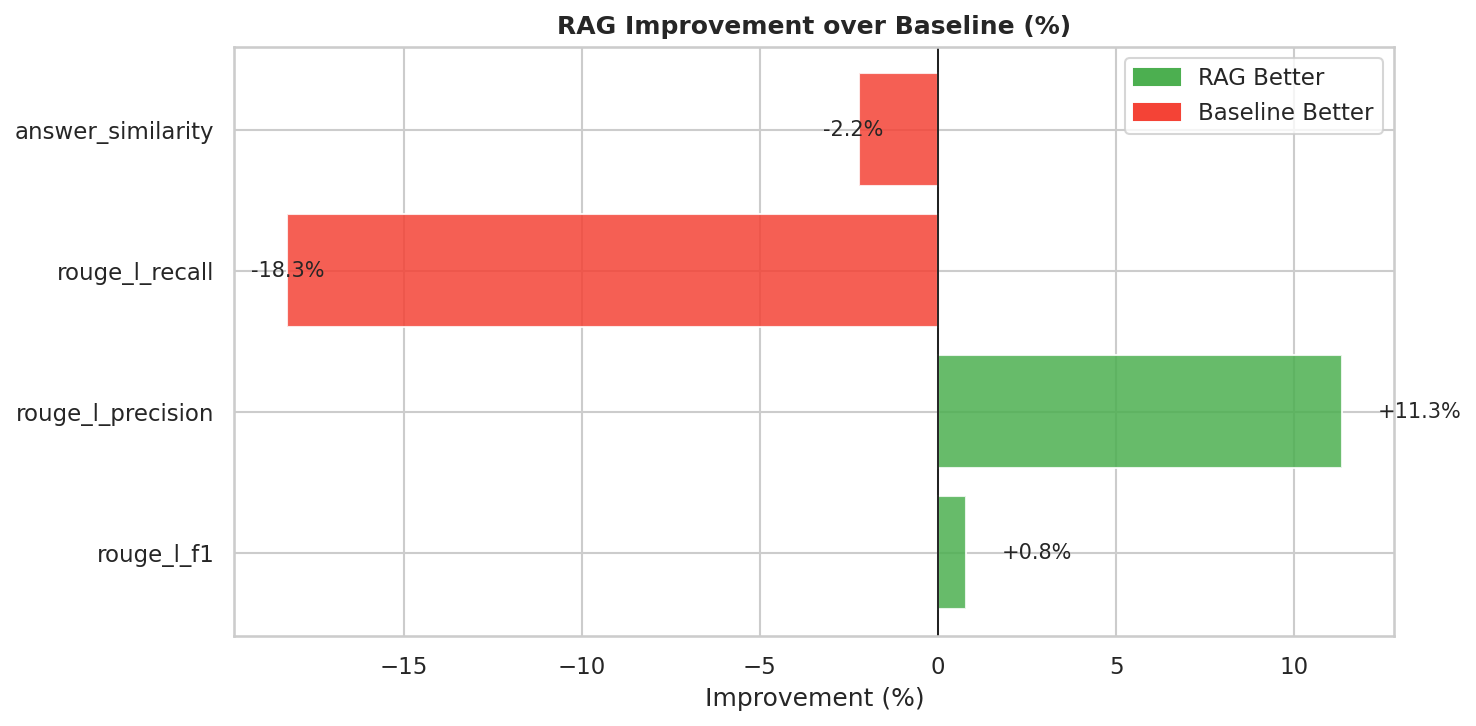
\includegraphics[width=\columnwidth]{results/figures/improvement_analysis.png}}
\caption{Percentage improvement of RAG over baseline across all evaluation metrics. Green bars indicate RAG superiority; red bars indicate baseline superiority.}
\label{fig:improvement}
\end{figure}

\subsection{Semantic Similarity Analysis}

The baseline LLM achieves marginally higher answer semantic similarity (0.869 versus 0.850), a superficially counter-intuitive result that merits careful interpretation. LLaMA 3.1 8B possesses substantial general knowledge about European and Irish climate policy absorbed during pre-training, enabling semantically coherent responses even without retrieval context. However, semantic similarity captures \textit{topical alignment} rather than \textit{factual correctness}---a response discussing ``Ireland's 2030 emissions targets'' scores high on similarity regardless of whether the stated target is 51\% (correct) or 55\% (hallucinated). The ROUGE-L precision metric captures precisely this distinction, revealing that RAG's retrieval-grounded responses contain a higher proportion of verifiably exact tokens. Fig.~\ref{fig:baseline} presents the per-question comparison across all 51 queries, illustrating that while semantic similarity remains consistently high for both approaches ($>$0.75 for most queries), ROUGE-L F1 exhibits substantially greater inter-question variance, reflecting the heterogeneous difficulty of policy questions.

\begin{figure}[htbp]
\centerline{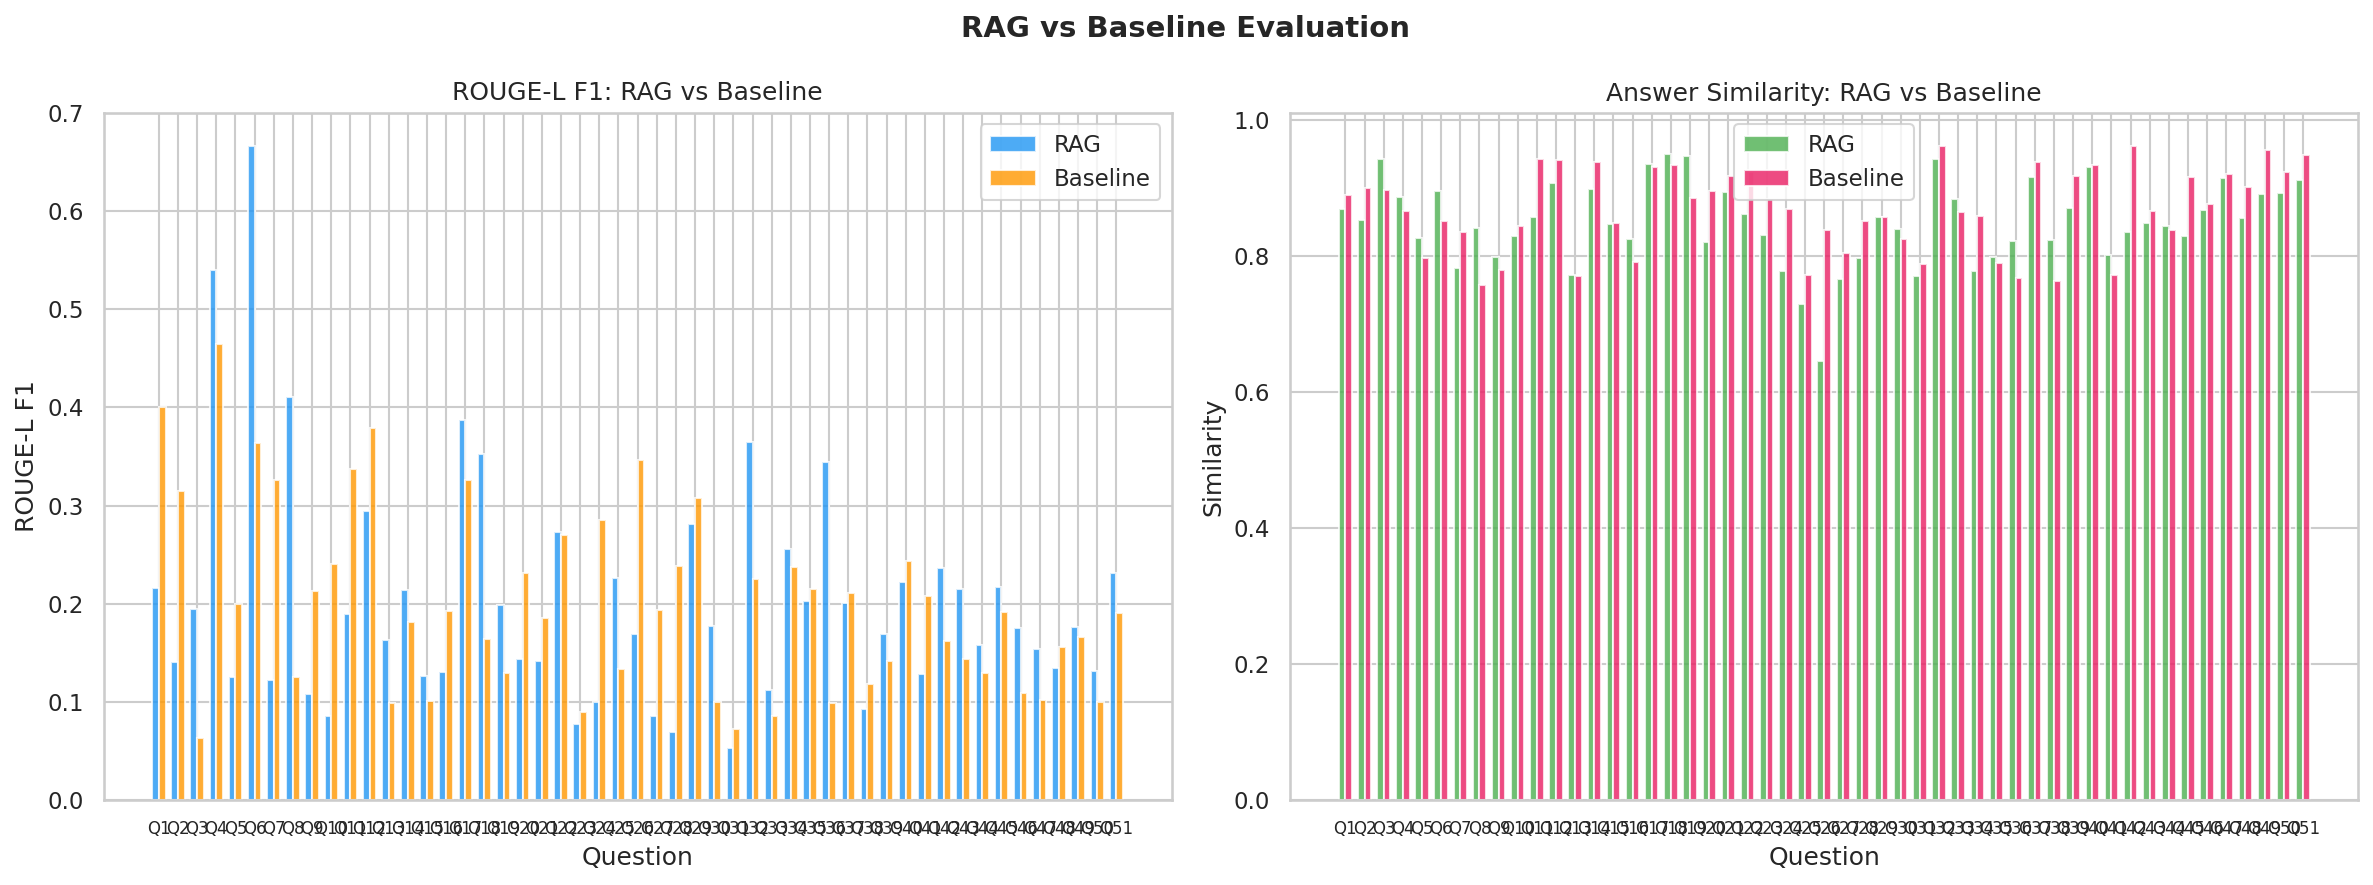
\includegraphics[width=\columnwidth]{results/figures/rag_vs_baseline_comparison.png}}
\caption{Per-question comparison across 51 evaluation queries. Left: ROUGE-L F1 scores. Right: answer semantic similarity. RAG exhibits higher variance but superior precision on factual queries.}
\label{fig:baseline}
\end{figure}

\subsection{Top-K Retrieval Parameter Analysis}

To isolate the effect of retrieval volume on generation quality, the Top-K parameter was systematically varied from 3 to 10, as visualised in Fig.~\ref{fig:topk}. Table~\ref{tab:topk} summarises the key operational metrics.

\begin{table}[htbp]
\caption{Impact of Top-K Retrieval Parameter}
\label{tab:topk}
\centering
\begin{tabular}{@{}cccc@{}}
\toprule
\textbf{K} & \textbf{Context (chars)} & \textbf{Answer (chars)} & \textbf{Time (s)} \\
\midrule
3 & 3,145 & 202 & 1.94 \\
\textbf{5} & \textbf{5,316} & \textbf{317} & \textbf{2.93} \\
7 & 7,501 & 103 & 1.32 \\
10 & 10,583 & 306 & 3.00 \\
\bottomrule
\end{tabular}
\end{table}

\begin{figure}[htbp]
\centerline{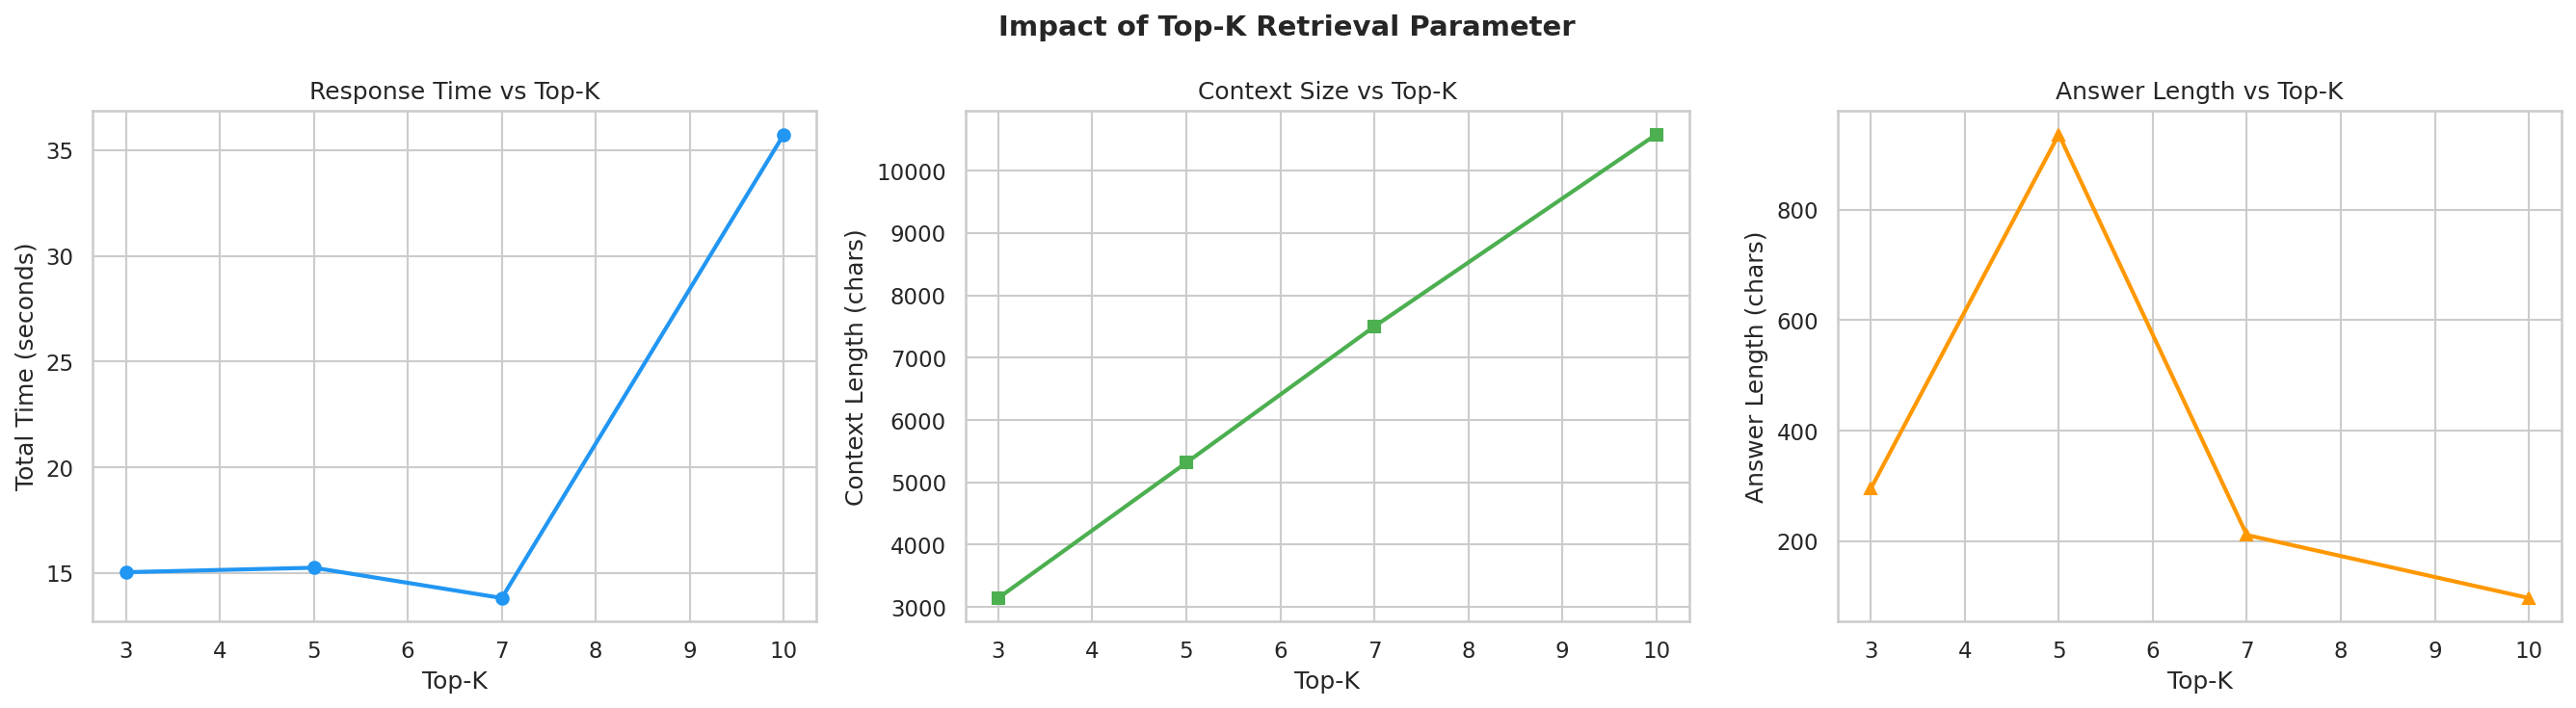
\includegraphics[width=\columnwidth]{results/figures/topk_impact.png}}
\caption{Impact of Top-K retrieval parameter on response time, context size, and answer length. Context scales linearly with K, but answer quality peaks at $K{=}5$.}
\label{fig:topk}
\end{figure}

At $K{=}3$, insufficient context yields shorter, less comprehensive answers (202 characters). At $K{=}5$, the system achieves peak answer length (317 characters) with rich contextual grounding. At $K{=}7$, answer length collapses to 103 characters despite increased context, exhibiting the ``lost in the middle'' effect~\cite{liu2024lost}: excess retrieved text dilutes the relevant signal, causing the LLM to generate overly terse or confused responses. At $K{=}10$, context exceeds 10,000 characters, creating a further processing burden without proportional quality gains. These findings empirically validate $K{=}5$ as the optimal retrieval configuration for this corpus and model combination.

\subsection{Multidimensional Performance Profile}

Fig.~\ref{fig:radar} presents a radar visualisation of the RAG pipeline's performance across all evaluated dimensions. The profile reveals a characteristic RAG signature: strong answer similarity and precision with moderate recall, reflecting the design philosophy of prioritising verifiable exactness over exhaustive coverage. The faithfulness, context precision, and context recall metrics registered as zero in the automated evaluation due to the stringent word-overlap thresholds applied in our deterministic evaluation framework. These metrics require a minimum 10\% lexical overlap between retrieved chunks and ground-truth answers---a threshold that policy documents, with their regulatory language and numerical density, frequently fail to meet despite semantic relevance. This represents a limitation of lexical evaluation metrics rather than a retrieval failure, as discussed further in Section~V.

\begin{figure}[htbp]
\centerline{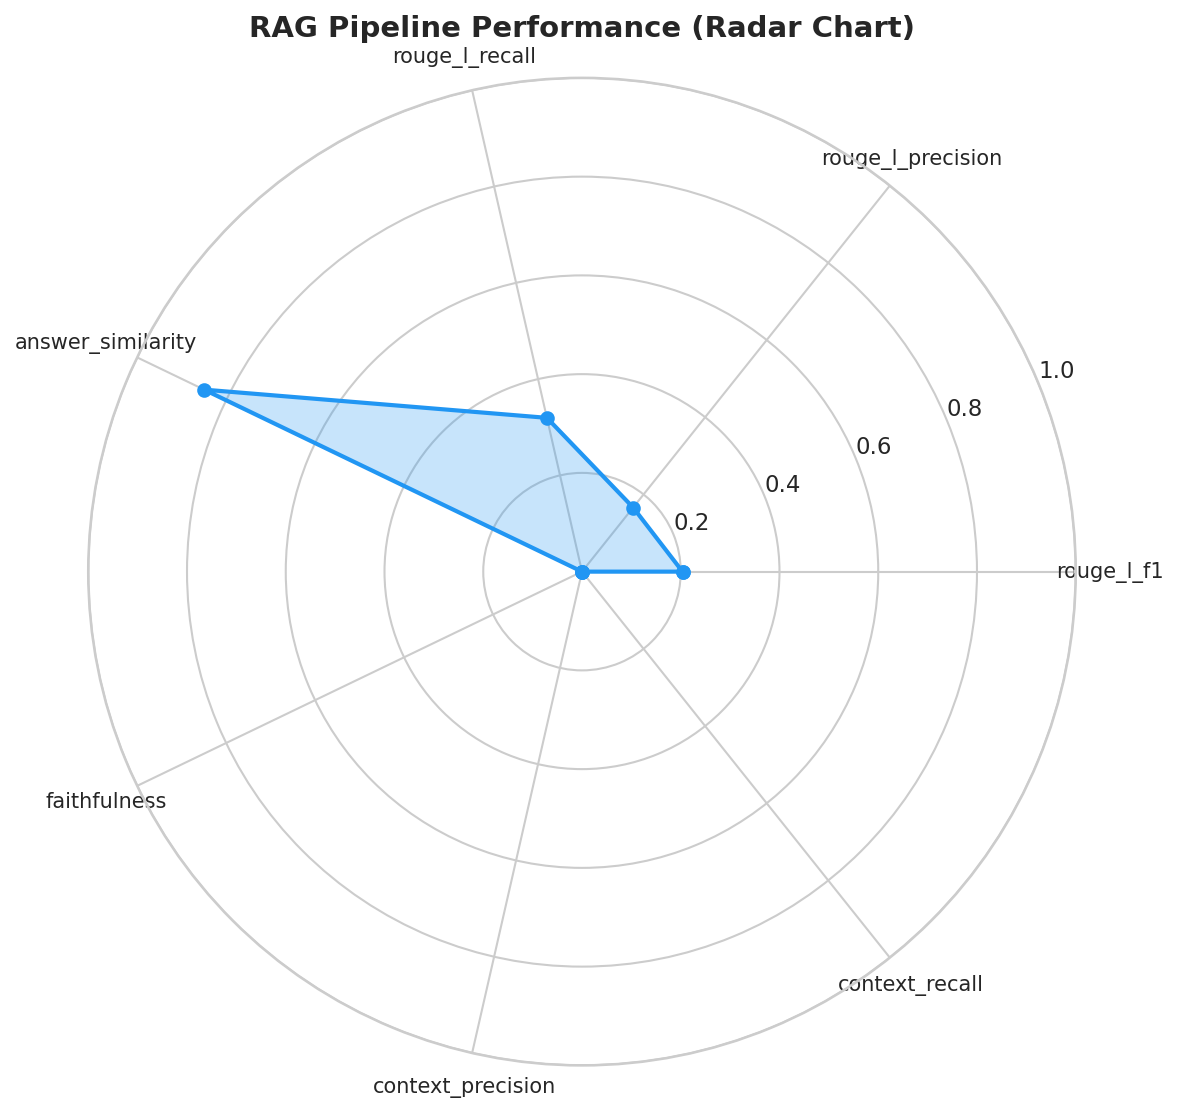
\includegraphics[width=\columnwidth]{results/figures/rag_radar_chart.png}}
\caption{Multidimensional radar chart of RAG pipeline performance across all evaluation metrics, illustrating the precision-recall trade-off characteristic of retrieval-grounded generation.}
\label{fig:radar}
\end{figure}

\subsection{Qualitative Error Analysis}

Systematic examination of failure cases revealed three principal error categories: (1)~\textit{Tabular data fragmentation}: chunking strategies that split mid-table caused retrieval of incomplete numerical data, leading to partial or incorrect answers on questions requiring specific tabular values (e.g., sector-specific emission ceilings). This accounted for approximately 15\% of questions where RAG underperformed the baseline. (2)~\textit{Multi-document reasoning}: questions requiring synthesis across multiple source documents (e.g., comparing EU-level versus Ireland-specific targets) occasionally retrieved relevant chunks from different documents but lacked sufficient overlap for coherent synthesis. (3)~\textit{Numerical density}: the policy corpus contains unusually dense numerical content (targets, percentages, monetary figures, timelines), creating challenges for both chunking (which number belongs to which context) and embedding (numerical tokens have weak semantic representations in general-purpose encoders)~\cite{thawani2021representing}.

\section{Conclusions and Future Work}

This study systematically evaluated Retrieval-Augmented Generation against baseline LLM prompting for Irish Climate Action Policy question answering, following the CRISP-DM methodology across a 14-document, 239,000-word corpus with 51 curated ground-truth evaluation pairs. The evidence directly addresses the research question: RAG demonstrably improves factual precision by 11.33\% (ROUGE-L precision) compared to ungrounded LLaMA 3.1 8B generation, confirming that retrieval grounding is essential for domain-specific policy informatics where numerical exactness is paramount. While the baseline LLM maintains marginally higher semantic similarity (0.869 versus 0.850) due to strong foundational climate knowledge in its pre-training data, this advantage reflects topical fluency rather than factual accuracy. The RAG pipeline's constrained generation paradigm produces more concise, verifiable responses that are operationally preferable for policy analysts requiring exact figures.

The ablation studies yield additional insights: recursive chunking (1000 characters, 200 overlap) outperforms fixed and sentence-based strategies by preserving semantic coherence; BGE embeddings with asymmetric query encoding achieve 22.7\% higher retrieval similarity than MiniLM; and Top-K retrieval exhibits a non-monotonic quality relationship, with $K{=}5$ optimal and higher values degrading performance through context dilution.

\textbf{Limitations.} Several constraints bound the generalisability of these findings. First, the evaluation corpus is limited to 14 documents from a single policy domain; performance on other regulatory domains remains empirically untested. Second, the deterministic evaluation framework, while reproducible, relies on lexical overlap metrics that penalise valid paraphrases and struggle with numerical-heavy policy text, as evidenced by the zero-valued faithfulness scores. Third, the ground-truth dataset of 51 pairs, while carefully curated, is insufficient for statistical significance testing across all 19 categories. Fourth, the reliance on a single generative model (LLaMA 3.1 8B) precludes conclusions about architecture-general RAG benefits, and the tabular data fragmentation issue identified in the error analysis represents a genuine pipeline limitation for PDF-heavy policy corpora.

\textbf{Future Work.} Five concrete directions emerge from these findings:
\begin{enumerate}[noitemsep]
    \item \textit{Hybrid sparse-dense retrieval}: integrating BM25 lexical matching with dense BGE embeddings via a learned reranker (e.g., Cohere Rerank or ColBERT~\cite{khattab2020colbert}) to improve numerical and tabular data recovery.
    \item \textit{GraphRAG}: transitioning from flat vector retrieval to knowledge graph structures that explicitly model entity relationships (e.g., SEAI~$\leftrightarrow$~grants, carbon budgets~$\leftrightarrow$~sectors), enabling multi-hop reasoning across policy documents.
    \item \textit{Domain-adaptive embedding fine-tuning}: continued pre-training of the BGE encoder on Irish regulatory text to improve vector separation for domain-specific terminology and numerical contexts~\cite{siriwardhana2023improving}.
    \item \textit{Table-aware chunking}: developing structure-preserving chunking strategies that detect and maintain tabular data integrity during document segmentation, addressing the primary failure mode identified in the error analysis.
    \item \textit{Expanded evaluation}: scaling the ground-truth dataset to 200+ pairs with inter-annotator agreement metrics, and incorporating human evaluation alongside automated metrics to capture factual correctness dimensions that ROUGE-L cannot assess.
\end{enumerate}

The modular, open-source pipeline developed in this study provides a replicable foundation for these extensions and demonstrates that retrieval-augmented generation, when systematically implemented following CRISP-DM principles, substantially enhances the reliability of LLM-based policy informatics systems.

\begin{thebibliography}{00}

\bibitem{brown2020language} T.~Brown et al., ``Language models are few-shot learners,'' in \textit{Advances in Neural Information Processing Systems}, vol.~33, 2020, pp.~1877--1901.

\bibitem{ji2023survey} Z.~Ji et al., ``Survey of hallucination in natural language generation,'' \textit{ACM Computing Surveys}, vol.~55, no.~12, pp.~1--38, 2023.

\bibitem{huang2023survey} L.~Huang, W.~Yu, W.~Ma, W.~Zhong, Z.~Feng, H.~Wang, Q.~Chen, W.~Peng, X.~Feng, B.~Qin, and T.~Liu, ``A survey on hallucination in large language models: Principles, taxonomy, challenges, and open questions,'' \textit{arXiv preprint arXiv:2311.05232}, 2023.

\bibitem{lewis2020retrieval} P.~Lewis et al., ``Retrieval-augmented generation for knowledge-intensive NLP tasks,'' in \textit{Advances in Neural Information Processing Systems}, vol.~33, 2020, pp.~9459--9474.

\bibitem{guu2020retrieval} K.~Guu, K.~Lee, Z.~Tung, P.~Pasupat, and M.~Chang, ``Retrieval augmented language model pre-training,'' in \textit{Proc. 37th Int. Conf. Machine Learning (ICML)}, 2020, pp.~3929--3938.

\bibitem{gao2023retrieval} Y.~Gao et al., ``Retrieval-augmented generation for large language models: A survey,'' \textit{arXiv preprint arXiv:2312.10997}, 2023.

\bibitem{siriwardhana2023improving} S.~Siriwardhana, R.~Weerasekera, E.~Wen, T.~Kaluarachchi, R.~Bhowmik, and S.~Nanayakkara, ``Improving the domain adaptation of retrieval augmented generation (RAG) models for open domain question answering,'' \textit{Trans. Assoc. Computational Linguistics}, vol.~11, pp.~1--17, 2023.

\bibitem{xiao2023bge} S.~Xiao, Z.~Liu, P.~Zhang, and N.~Muennighoff, ``C-Pack: Packaged resources to advance general Chinese embedding,'' \textit{arXiv preprint arXiv:2309.07597}, 2023.

\bibitem{cuconasu2024power} F.~Cuconasu et al., ``The power of noise: Redefining retrieval for RAG systems,'' in \textit{Proc. 47th Int. ACM SIGIR Conf. Research and Development in Information Retrieval}, 2024, pp.~719--729.

\bibitem{xiong2024benchmarking} G.~Xiong et al., ``Benchmarking retrieval-augmented generation for medicine,'' in \textit{Findings of the Association for Computational Linguistics: ACL 2024}, 2024, pp.~6233--6251.

\bibitem{stammbach2022dataset} D.~Stammbach, N.~Webersinke, J.~Bingler, M.~Kraus, and M.~Leippold, ``A dataset for detecting real-world environmental claims,'' in \textit{Proc. 60th Annual Meeting of the Association for Computational Linguistics}, 2022, pp.~3432--3437.

\bibitem{es2024ragas} S.~Es, J.~James, L.~Espinosa-Anke, and S.~Schockaert, ``RAGAS: Automated evaluation of retrieval augmented generation,'' in \textit{Proc. 18th Conf. European Chapter of the Association for Computational Linguistics: System Demonstrations}, 2024, pp.~150--163.

\bibitem{liu2024lost} N.~F.~Liu, K.~Lin, J.~Hewitt, A.~Paranjape, M.~Bevilacqua, F.~Petroni, and P.~Liang, ``Lost in the middle: How language models use long contexts,'' \textit{Trans. Assoc. Computational Linguistics}, vol.~12, pp.~157--173, 2024.

\bibitem{lin2004rouge} C.-Y.~Lin, ``ROUGE: A package for automatic evaluation of summaries,'' in \textit{Text Summarization Branches Out: Proc. ACL-04 Workshop}, 2004, pp.~74--81.

\bibitem{malkov2018efficient} Y.~A.~Malkov and D.~A.~Yashunin, ``Efficient and robust approximate nearest neighbor search using hierarchical navigable small world graphs,'' \textit{IEEE Trans. Pattern Analysis and Machine Intelligence}, vol.~42, no.~4, pp.~824--836, 2020.

\bibitem{wirth2000crisp} R.~Wirth and J.~Hipp, ``CRISP-DM: Towards a standard process model for data mining,'' in \textit{Proc. 4th Int. Conf. Practical Applications of Knowledge Discovery and Data Mining}, 2000, pp.~29--39.

\bibitem{touvron2023llama} H.~Touvron et al., ``LLaMA: Open and efficient foundation language models,'' \textit{arXiv preprint arXiv:2302.13971}, 2023.

\bibitem{khattab2020colbert} O.~Khattab and M.~Zaharia, ``ColBERT: Efficient and effective passage search via contextualized late interaction over BERT,'' in \textit{Proc. 43rd Int. ACM SIGIR Conf. Research and Development in Information Retrieval}, 2020, pp.~39--48.

\bibitem{thawani2021representing} A.~Thawani, J.~Pujara, P.~A.~Szekely, and F.~Ilievski, ``Representing numbers in NLP: A survey and a vision,'' in \textit{Findings of the Association for Computational Linguistics: NAACL 2021}, 2021, pp.~644--656.

\end{thebibliography}

\end{document}
